% ============================================================================
%  RetailAPOLLO -- simple data flow
%  Compile:  pdflatex DATA_FLOW.tex     (one landscape page)
% ============================================================================
\documentclass[11pt]{article}
\usepackage[T1]{fontenc}
\usepackage[paperwidth=42cm,paperheight=34cm,margin=1.0cm]{geometry}
\usepackage{tikz}
\usepackage{xcolor}
\usetikzlibrary{arrows.meta,positioning,calc}
\pagestyle{empty}
\setlength{\parindent}{0pt}

\definecolor{cSrc}{HTML}{1F4E79}\definecolor{cSrcBg}{HTML}{DCE9F5}
\definecolor{cStep}{HTML}{7B2D26}\definecolor{cStepBg}{HTML}{F8E0DD}
\definecolor{cSam}{HTML}{7A5C00}\definecolor{cSamBg}{HTML}{FCF4DC}
\definecolor{cOut}{HTML}{1E5B45}\definecolor{cOutBg}{HTML}{DDF0E6}
\definecolor{cNote}{HTML}{666666}\definecolor{cNoteBg}{HTML}{F2F2F2}

\newcommand{\cd}[1]{{\ttfamily\small\detokenize{#1}}}
\newcommand{\cdt}[1]{{\ttfamily\scriptsize\detokenize{#1}}}

\tikzset{
  box/.style={draw,rounded corners=3pt,line width=0.9pt,align=left,
              inner sep=8pt,anchor=north west,font=\normalsize},
  src/.style ={box,draw=cSrc, fill=cSrcBg, text width=#1},
  step/.style={box,draw=cStep,fill=cStepBg,text width=#1,line width=1.4pt},
  sam/.style ={box,draw=cSam, fill=cSamBg, text width=#1},
  out/.style ={box,draw=cOut, fill=cOutBg, text width=#1,line width=1.4pt},
  note/.style={box,draw=cNote,fill=cNoteBg,dashed,text width=#1,font=\small},
  flow/.style={-{Latex[length=5mm,width=4mm]},line width=2.2pt,draw=black!65},
  hint/.style={-{Latex[length=3.5mm,width=2.6mm]},line width=1.0pt,draw=black!50,dashed},
}

\begin{document}
\begin{center}
{\huge\bfseries RetailAPOLLO --- how the data gets in}\\[3pt]
{\large Pull $\rightarrow$ keep compressed $\rightarrow$ turn into tables $\rightarrow$ clean \& count $\rightarrow$ use}
\end{center}
\vspace{2mm}

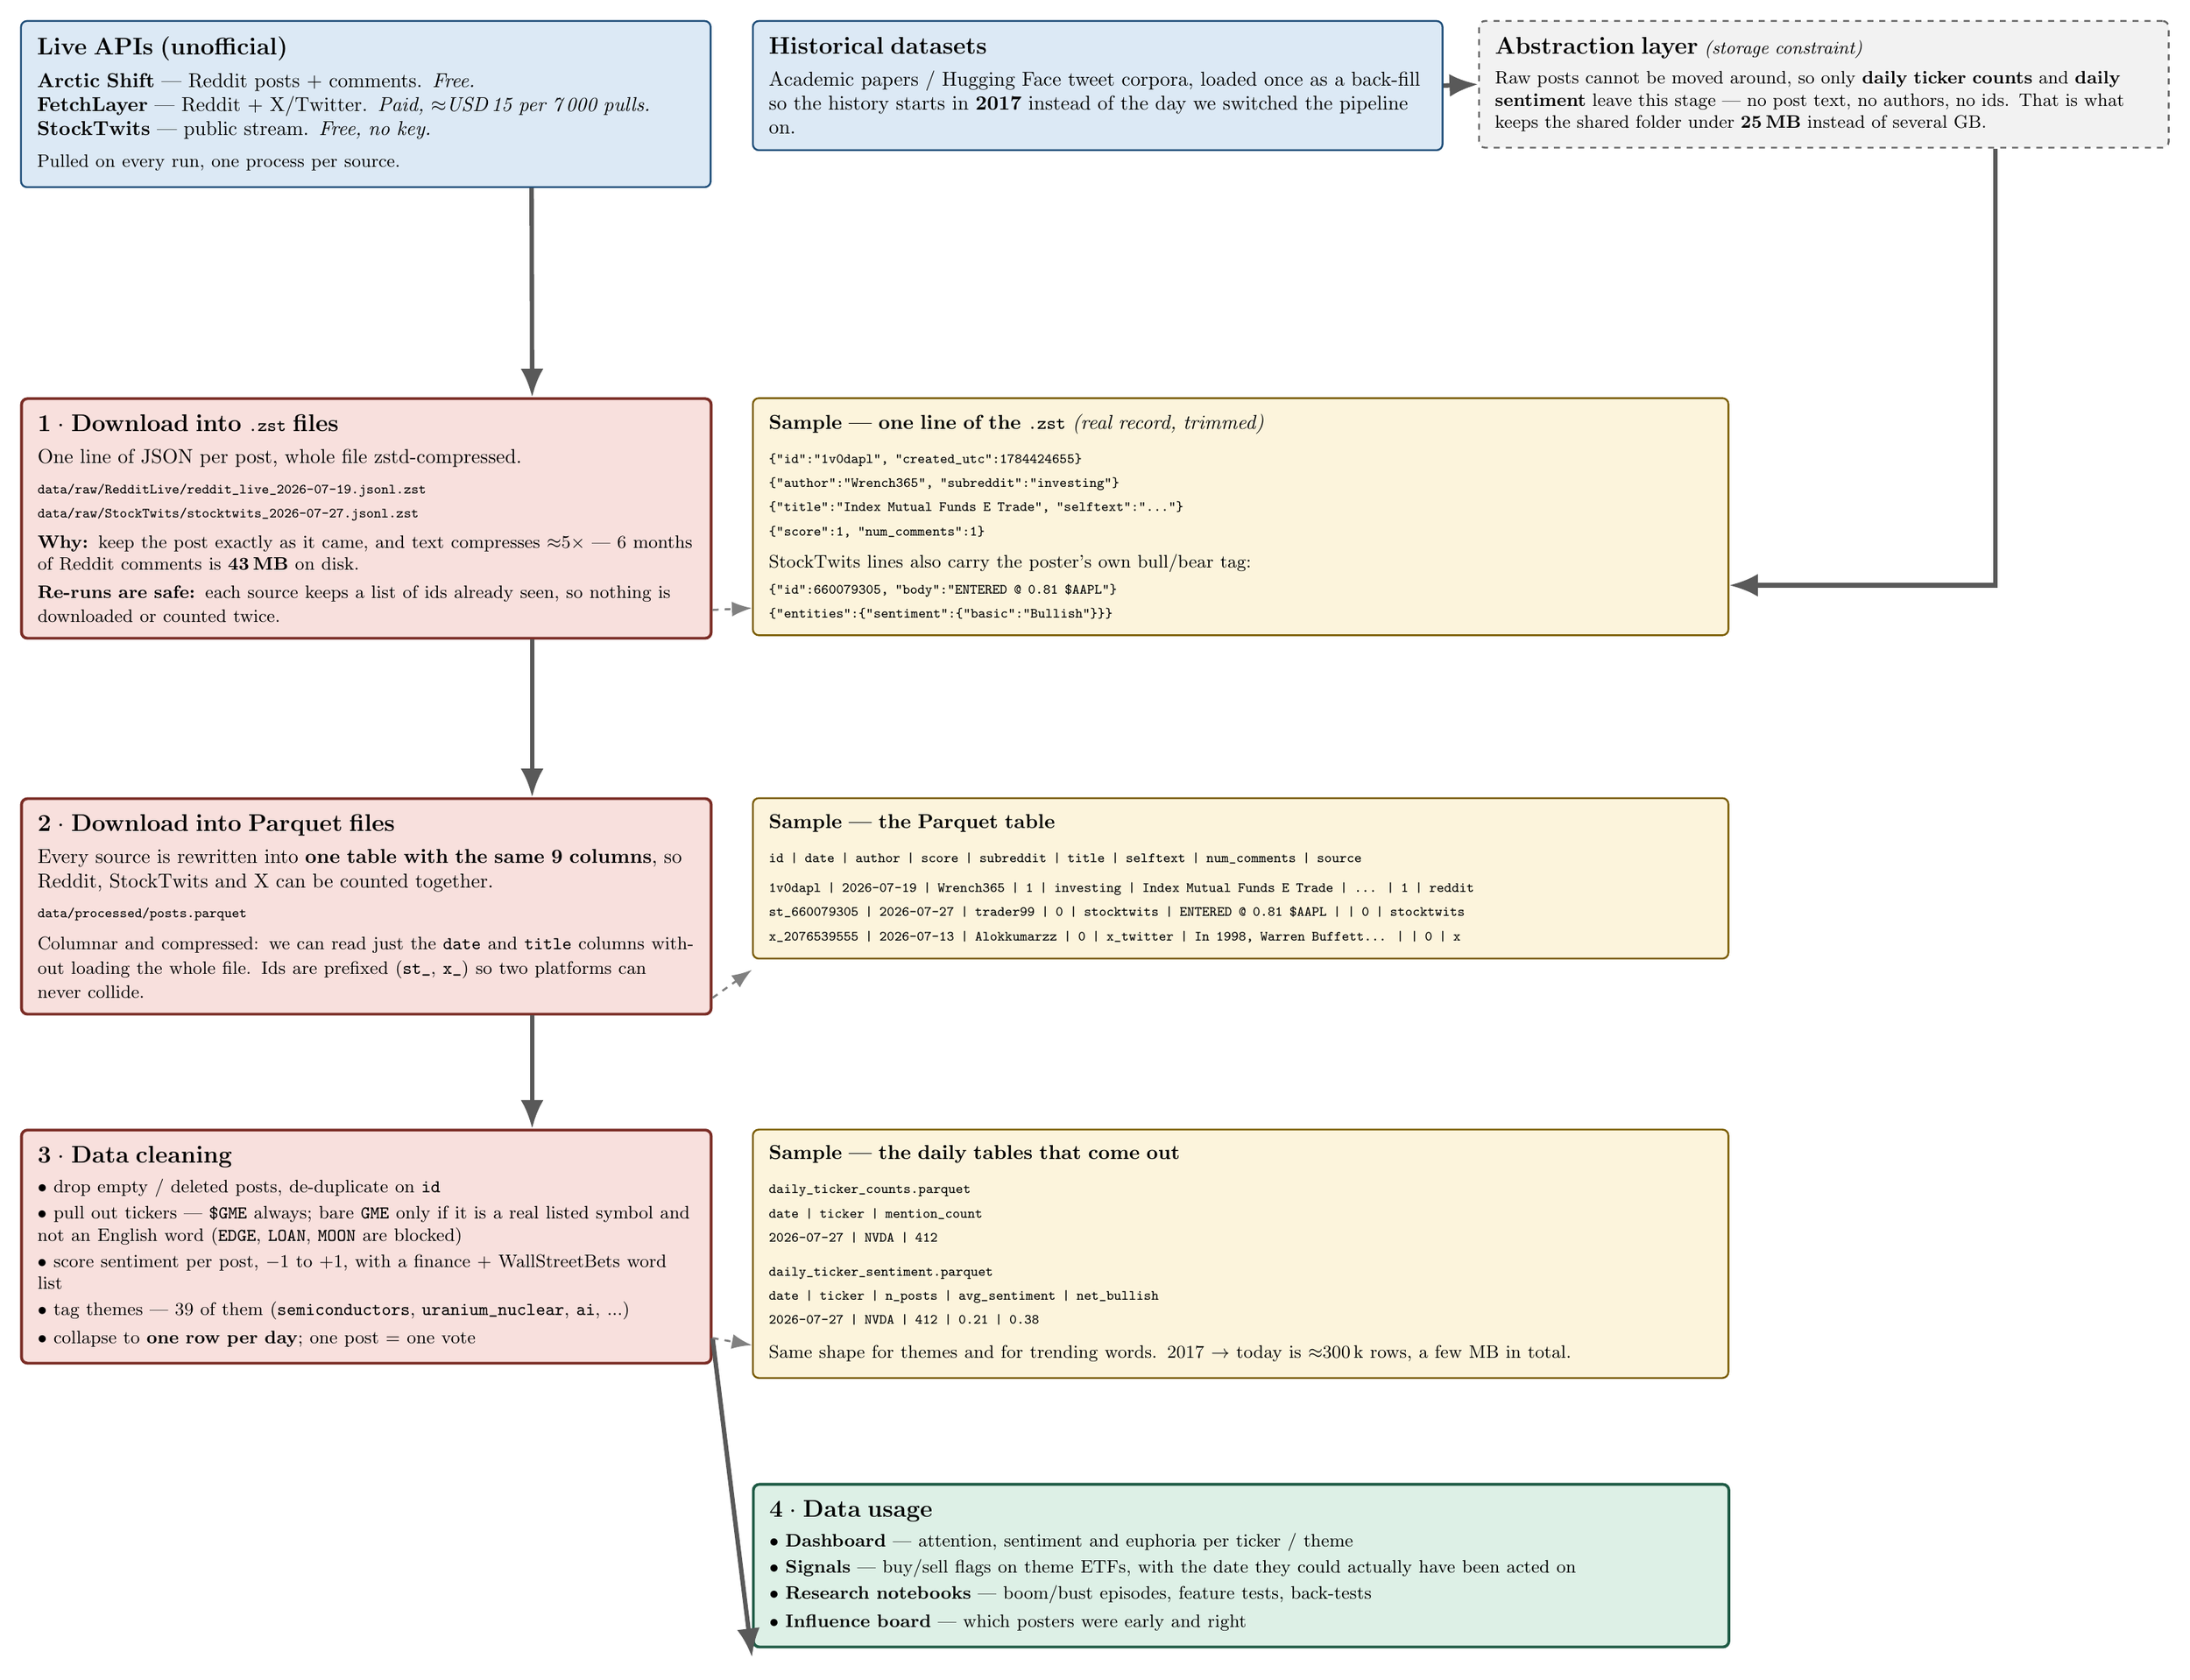
\begin{tikzpicture}[x=1cm,y=1cm]

% ---------------------------------------------------------------- SOURCES
\node[src=11.5cm] (api) at (0,0) {%
\textbf{\large Live APIs (unofficial)}\\[4pt]
\textbf{Arctic Shift} --- Reddit posts + comments. \emph{Free.}\\
\textbf{FetchLayer} --- Reddit + X/Twitter. \emph{Paid,
$\approx$USD\,15 per 7\,000 pulls.}\\
\textbf{StockTwits} --- public stream. \emph{Free, no key.}\\[4pt]
\small Pulled on every run, one process per source.};

\node[src=11.5cm] (hist) at (12.8,0) {%
\textbf{\large Historical datasets}\\[4pt]
Academic papers / Hugging Face tweet corpora, loaded once as a
back-fill so the history starts in \textbf{2017} instead of the day
we switched the pipeline on.};

\node[note=11.5cm] (abs) at (25.5,0) {%
\textbf{\large Abstraction layer} \emph{(storage constraint)}\\[4pt]
Raw posts cannot be moved around, so only \textbf{daily ticker counts}
and \textbf{daily sentiment} leave this stage --- no post text, no
authors, no ids. That is what keeps the shared folder under
\textbf{25\,MB} instead of several GB.};

% ---------------------------------------------------------------- STEP 1
\node[step=11.5cm] (s1) at (0,-6.6) {%
\textbf{\large 1 $\cdot$ Download into \cd{.zst} files}\\[4pt]
One line of JSON per post, whole file zstd-compressed.\\[3pt]
\cdt{data/raw/RedditLive/reddit_live_2026-07-19.jsonl.zst}\\
\cdt{data/raw/StockTwits/stocktwits_2026-07-27.jsonl.zst}\\[4pt]
\small \textbf{Why:} keep the post exactly as it came, and text
compresses $\approx$5$\times$ --- 6 months of Reddit comments is
\textbf{43\,MB} on disk.\\[2pt]
\textbf{Re-runs are safe:} each source keeps a list of ids already
seen, so nothing is downloaded or counted twice.};

\node[sam=16.5cm] (x1) at (12.8,-6.6) {%
\textbf{Sample --- one line of the \cd{.zst}} \emph{(real record, trimmed)}\\[5pt]
\cdt{{"id":"1v0dapl", "created_utc":1784424655}}\\
\cdt{{"author":"Wrench365", "subreddit":"investing"}}\\
\cdt{{"title":"Index Mutual Funds E Trade", "selftext":"..."}}\\
\cdt{{"score":1, "num_comments":1}}\\[5pt]
\small StockTwits lines also carry the poster's own bull/bear tag:\\[2pt]
\cdt{{"id":660079305, "body":"ENTERED @ 0.81 $AAPL"}}\\
\cdt{{"entities":{"sentiment":{"basic":"Bullish"}}}}};

% ---------------------------------------------------------------- STEP 2
\node[step=11.5cm] (s2) at (0,-13.6) {%
\textbf{\large 2 $\cdot$ Download into Parquet files}\\[4pt]
Every source is rewritten into \textbf{one table with the same
9 columns}, so Reddit, StockTwits and X can be counted together.\\[3pt]
\cdt{data/processed/posts.parquet}\\[4pt]
\small Columnar and compressed: we can read just the \cd{date} and
\cd{title} columns without loading the whole file. Ids are prefixed
(\cd{st_}, \cd{x_}) so two platforms can never collide.};

\node[sam=16.5cm] (x2) at (12.8,-13.6) {%
\textbf{Sample --- the Parquet table}\\[5pt]
\cdt{id | date | author | score | subreddit | title | selftext | num_comments | source}\\[3pt]
\cdt{1v0dapl | 2026-07-19 | Wrench365 | 1 | investing | Index Mutual Funds E Trade | ... | 1 | reddit}\\
\cdt{st_660079305 | 2026-07-27 | trader99 | 0 | stocktwits | ENTERED @ 0.81 $AAPL | | 0 | stocktwits}\\
\cdt{x_2076539555 | 2026-07-13 | Alokkumarzz | 0 | x_twitter | In 1998, Warren Buffett... | | 0 | x}};

% ---------------------------------------------------------------- STEP 3
\node[step=11.5cm] (s3) at (0,-19.4) {%
\textbf{\large 3 $\cdot$ Data cleaning}\\[4pt]
\small
$\bullet$ drop empty / deleted posts, de-duplicate on \cd{id}\\[2pt]
$\bullet$ pull out tickers --- \cd{$GME} always; bare \cd{GME} only if it
is a real listed symbol and not an English word
(\cd{EDGE}, \cd{LOAN}, \cd{MOON} are blocked)\\[2pt]
$\bullet$ score sentiment per post, $-1$ to $+1$, with a finance +
WallStreetBets word list\\[2pt]
$\bullet$ tag themes --- 39 of them (\cd{semiconductors},
\cd{uranium_nuclear}, \cd{ai}, ...)\\[2pt]
$\bullet$ collapse to \textbf{one row per day}; one post = one vote};

\node[sam=16.5cm] (x3) at (12.8,-19.4) {%
\textbf{Sample --- the daily tables that come out}\\[5pt]
\cdt{daily_ticker_counts.parquet}\\
\cdt{date | ticker | mention_count}\\
\cdt{2026-07-27 | NVDA | 412}\\[5pt]
\cdt{daily_ticker_sentiment.parquet}\\
\cdt{date | ticker | n_posts | avg_sentiment | net_bullish}\\
\cdt{2026-07-27 | NVDA | 412 | 0.21 | 0.38}\\[5pt]
\small Same shape for themes and for trending words.
2017 $\rightarrow$ today is $\approx$300\,k rows, a few MB in total.};

% ---------------------------------------------------------------- STEP 4
\node[out=16.5cm] (s4) at (12.8,-25.6) {%
\textbf{\large 4 $\cdot$ Data usage}\\[4pt]
\small
$\bullet$ \textbf{Dashboard} --- attention, sentiment and euphoria per ticker / theme\\[2pt]
$\bullet$ \textbf{Signals} --- buy/sell flags on theme ETFs, with the date they could
actually have been acted on\\[2pt]
$\bullet$ \textbf{Research notebooks} --- boom/bust episodes, feature tests, back-tests\\[2pt]
$\bullet$ \textbf{Influence board} --- which posters were early and right};

% ---------------------------------------------------------------- arrows
\draw[flow] ($(api.south)+(2.9,0)$) -- ($(s1.north)+(2.9,0)$);
\draw[flow] ($(s1.south)+(2.9,0)$) -- ($(s2.north)+(2.9,0)$);
\draw[flow] ($(s2.south)+(2.9,0)$) -- ($(s3.north)+(2.9,0)$);
\draw[flow] ($(s3.east)+(0,-1.6)$) -- ($(s4.west)+(0,-1.6)$);

\draw[flow] (hist.east) -- (abs.west);
\draw[flow] ($(abs.south)+(3.0,0)$) |- ($(x1.east)+(0,-1.2)$);

\draw[hint] ($(s1.east)+(0,-1.6)$) -- ($(x1.west)+(0,-1.6)$);
\draw[hint] ($(s2.east)+(0,-1.6)$) -- ($(x2.west)+(0,-1.6)$);
\draw[hint] ($(s3.east)+(0,-1.6)$) -- ($(x3.west)+(0,-1.6)$);

\end{tikzpicture}
\end{document}
